% This is "sig-alternate.tex" V1.9 April 2009
% This file should be compiled with V2.4 of "sig-alternate.cls" April 2009
%
% This example file demonstrates the use of the 'sig-alternate.cls'
% V2.4 LaTeX2e document class file. It is for those submitting
% articles to ACM Conference Proceedings WHO DO NOT WISH TO
% STRICTLY ADHERE TO THE SIGS (PUBS-BOARD-ENDORSED) STYLE.
% The 'sig-alternate.cls' file will produce a similar-looking,
% albeit, 'tighter' paper resulting in, invariably, fewer pages.
%
% ----------------------------------------------------------------------------------------------------------------
% This .tex file (and associated .cls V2.4) produces:
%       1) The Permission Statement
%       2) The Conference (location) Info information
%       3) The Copyright Line with ACM data
%       4) NO page numbers
%
% as against the acm_proc_article-sp.cls file which
% DOES NOT produce 1) thru' 3) above.
%
% Using 'sig-alternate.cls' you have control, however, from within
% the source .tex file, over both the CopyrightYear
% (defaulted to 200X) and the ACM Copyright Data
% (defaulted to X-XXXXX-XX-X/XX/XX).
% e.g.
% \CopyrightYear{2007} will cause 2007 to appear in the copyright line.
% \crdata{0-12345-67-8/90/12} will cause 0-12345-67-8/90/12 to appear in the copyright line.
%
% ---------------------------------------------------------------------------------------------------------------
% This .tex source is an example which *does* use
% the .bib file (from which the .bbl file % is produced).
% REMEMBER HOWEVER: After having produced the .bbl file,
% and prior to final submission, you *NEED* to 'insert'
% your .bbl file into your source .tex file so as to provide
% ONE 'self-contained' source file.
%
% ================= IF YOU HAVE QUESTIONS =======================
% Questions regarding the SIGS styles, SIGS policies and
% procedures, Conferences etc. should be sent to
% Adrienne Griscti (griscti@acm.org)
%
% Technical questions _only_ to
% Gerald Murray (murray@hq.acm.org)
% ===============================================================
%
% For tracking purposes - this is V1.9 - April 2009

\documentclass{sig-alternate}

\begin{document}
%
% --- Author Metadata here ---
\conferenceinfo{ICCAD}{'09 San Jose, CA USA}
\CopyrightYear{2009} % Allows default copyright year (200X) to be over-ridden - IF NEED BE.
\crdata{978-1-60558-800-1/09/11}  % Allows default copyright data (0-89791-88-6/97/05) to be over-ridden - IF NEED BE.
% --- End of Author Metadata ---

\title{Synthesizing Complementary Circuits Automatically}
%\subtitle{[Extended Abstract]
%\titlenote{A full version of this paper is available as
%\textit{Author's Guide to Preparing ACM SIG Proceedings Using
%\LaTeX$2_\epsilon$\ and BibTeX} at
%\texttt{www.acm.org/eaddress.htm}}}
%
% You need the command \numberofauthors to handle the 'placement
% and alignment' of the authors beneath the title.
%
% For aesthetic reasons, we recommend 'three authors at a time'
% i.e. three 'name/affiliation blocks' be placed beneath the title.
%
% NOTE: You are NOT restricted in how many 'rows' of
% "name/affiliations" may appear. We just ask that you restrict
% the number of 'columns' to three.
%
% Because of the available 'opening page real-estate'
% we ask you to refrain from putting more than six authors
% (two rows with three columns) beneath the article title.
% More than six makes the first-page appear very cluttered indeed.
%
% Use the \alignauthor commands to handle the names
% and affiliations for an 'aesthetic maximum' of six authors.
% Add names, affiliations, addresses for
% the seventh etc. author(s) as the argument for the
% \additionalauthors command.
% These 'additional authors' will be output/set for you
% without further effort on your part as the last section in
% the body of your article BEFORE References or any Appendices.

\numberofauthors{4} %  in this sample file, there are a *total*
% of EIGHT authors. SIX appear on the 'first-page' (for formatting
% reasons) and the remaining two appear in the \additionalauthors section.
%
\author{
% You can go ahead and credit any number of authors here,
% e.g. one 'row of three' or two rows (consisting of one row of three
% and a second row of one, two or three).
%
% The command \alignauthor (no curly braces needed) should
% precede each author name, affiliation/snail-mail address and
% e-mail address. Additionally, tag each line of
% affiliation/address with \affaddr, and tag the
% e-mail address with \email.
%
% 1st. author
\alignauthor
%Ben Trovato\titlenote{Dr.~Trovato insisted his name be first.}\\
ShengYu Shen\\
       \affaddr{School of Computer Science, National University of Defense Technology}\\
       \affaddr{410073,DeYa Avenue}\\
       \affaddr{ChangSha,China}\\
       \email{syshen@nudt.edu.cn}
% 2nd. author
\alignauthor
%G.K.M. Tobin\titlenote{The secretary disavows any knowledge of this author's actions.}\\
JianMin Zhang\\
       \affaddr{School of Computer Science, National University of Defense Technology}\\
       \affaddr{410073,DeYa Avenue}\\
       \affaddr{ChangSha,China}\\
       \email{jmzhang@nudt.edu.cn}
% 3rd. author
%\alignauthor Lars Th{\o}rv{\"a}ld\titlenote{This author is the one who did all the really hard work.}\\
\alignauthor
Ying Qin\\
       \affaddr{School of Computer Science, National University of Defense Technology}\\
       \affaddr{410073,DeYa Avenue}\\
       \affaddr{ChangSha,China}\\
       \email{qy123@nudt.edu.cn}
\and  % use '\and' if you need 'another row' of author names
% 4th. author
\alignauthor
%Lawrence P. Leipuner\\
SiKun Li\\
       \affaddr{School of Computer Science, National University of Defense Technology}\\
       \affaddr{410073,DeYa Avenue}\\
       \affaddr{ChangSha,China}\\
       \email{skli@nudt.edu.cn}
% 5th. author
%\alignauthor Sean Fogarty\\
%       \affaddr{NASA Ames Research Center}\\
%       \affaddr{Moffett Field}\\
%       \affaddr{California 94035}\\
%       \email{fogartys@amesres.org}
% 6th. author
%\alignauthor Charles Palmer\\
%       \affaddr{Palmer Research Laboratories}\\
%       \affaddr{8600 Datapoint Drive}\\
%       \affaddr{San Antonio, Texas 78229}\\
%       \email{cpalmer@prl.com}
}
% There's nothing stopping you putting the seventh, eighth, etc.
% author on the opening page (as the 'third row') but we ask,
% for aesthetic reasons that you place these 'additional authors'
% in the \additional authors block, viz.
%\additionalauthors{Additional authors: John Smith (The Th{\o}rv{\"a}ld Group,
%email: {\texttt{jsmith@affiliation.org}}) and Julius P.~Kumquat
%(The Kumquat Consortium, email: {\texttt{jpkumquat@consortium.net}}).}
%\date{30 July 1999}
% Just remember to make sure that the TOTAL number of authors
% is the number that will appear on the first page PLUS the
% number that will appear in the \additionalauthors section.

\maketitle
\begin{abstract}
One of the most difficult jobs in designing communication and multimedia chips,
is to design and verify complex complementary circuit pair $(E,E^{-1})$,
in which circuit $E$ transforms information into a format that is suitable for transmission and storage,
while $E$'s complementary circuit $E^{-1}$ recovers this information.

In order to ease this job,
we propose a novel two-step approach to synthesize complementary circuit $E^{-1}$ from $E$ fully automatically.
First, we assume that the circuit $E$ satisfies parameterized complementary assumption,
which means its input can be recovered from its output under some parameter setting.
We check this assumption with SAT solver and find out proper values of these parameters.
Second, with parameter values and the SAT instance obtained in the first step,
we build the complementary circuit $E^{-1}$ with an efficient satisfying assignments enumeration technique
that is specially designed for circuits with lots of XOR gates.

To illustrate its usefulness and efficiency,
we run our algorithm on several complex encoders from industrial projects,
including PCIE and 10G ethernet,
and successfully generate correct complementary circuits for them.
\end{abstract}

% A category with the (minimum) three required fields
%\category{H.4}{Information Systems Applications}{Miscellaneous}
%A category including the fourth, optional field follows...
%\category{D.2.8}{Software Engineering}{Metrics}[complexity measures, performance measures]
\category{B.5.2}{REGISTER-TRANSFER-LEVEL IMPLEMENTATION}{Design Aids}[Automatic synthesis]
\category{B.4.4}{ INPUT/OUTPUT AND DATA COMMUNICATIONS}{Performance Analysis and Design Aids}[Formal models]

\terms{Algorithms, Design, Theory, Verification}

\keywords{Synthesis,Complementary Circuit,Satisfying Assignments Enumeration} % NOT required for Proceedings

\section{Introduction}
Communication and multimedia electronic applications are major driving forces of semiconductor industry.
Many leading edge communication protocols and media formats,
even still in non-standardized draft status,
are implemented in chips and pushed to market,
to maximize the chance of being accepted by consumers and becoming the de facto standards.
Two such well known stories are the 802.11n wireless standard competition \cite{IEEE80211N},
and the disk format war between HD and blue ray \cite{BRHDVD}.
In such highly competitive markets,
designing correct chip as fast as possible is the key to success.

One of the most difficult jobs in designing communication and multimedia chips,
is to design and verify complex complementary circuit pair $(E,E^{-1})$,
in which circuit $E$ transforms information into a format that is suitable for transmission and storage,
while $E$'s complementary circuit $E^{-1}$ recovers this information.
Many factors significantly complicate the job of designing and verifying such circuit pairs.
For example, deep pipeline to achieve high frequency,
complex encoding mechanism to achieve reliability and compression ratio, and so on.

In order to ease this job,
we propose in this paper a novel approach to synthesize $E^{-1}$ from $E$ fully automatically in two steps.

\begin{enumerate}
  \item In the first step, we assume that,
        for $E$ under some parameters valuation,
	its input alphabet sequence can be uniquely determined by its output alphabet sequence.
	We call this assumption \textbf{parameterized complementary assumption}.
	We use a SAT solver to check this assumption and find out proper values for some parameters that make this assumption hold.
  \item In the second step,
        with the SAT instance and parameter values obtained in the first step,
	we build a circuit $E^{-1}$ with an efficient satisfying assignments enumeration technology(abbreviated as \textbf{ALLSAT}),
	which is specially designed for communication and arithmetic circuit with lots of XOR gates.
\end{enumerate}

We implement our algorithm on zchaff \cite{CHAFF},
and run it on several complex encoder circuits from industrial projects,
including PCIE and 10G Ethernet.
We can build complementary circuits for all of them within 3000 seconds.

\textbf{The contribution of this paper is twofold}:
1) We propose the first approach to decide if it's possible to recover input sequence of an circuit $E$ from its output sequence.
2) We propose an efficient ALLSAT algorithm for XOR intensive circuits,
to build complementary circuit $E^{-1}$ from the SAT instance of circuit $E$.

\textbf{The remainder of this paper is organized as follows}.
Section 2 presents background material.
Section 3 presents how to check parameterized complementary assumption,
and how to find out proper values of its parameters.
Section 4 presents how to build complementary circuit.
Section 5 presents experimental results of our approach.
Section 6 presents related works.
Section 7 concludes with a note on future work.


\section{Preliminaries}

\subsection{Propositional Satisfiability Problem}
For a boolean formula $F$ over variable set $V$,
the \textbf{Propositional Satisfiability Problem}(abbreviated as \textbf{SAT}) is to find an \textbf{satisfying assignment} $A:V\to \{0,1\}$,
such that $F$ can be evaluated to 1.

If such a satisfying assignment exists, then $F$ is called a \textbf{satisfiable formula},
%This problem is NP-complete in general,
%but some efficient SAT solver have been developed,
%such as zchaff\cite{CHAFF} ,Berkmin\cite{BERKMIN} and MiniSAT\cite{EXTSAT}.
otherwise it is called \textbf{unsatisfiable formula}.
%Unsatisfiable instance often has many subsets that are also unsatisfiable,
%these subsets are called \textbf{unsatisfiable core}.
%Many efficient unsatisfiable core extraction algorithms are proposed by researchers\cite{VERPROOF,VALIDSAT}.

A computer program that decides the existence of such satisfying assignment is called \textbf{SAT solver}.

For an assignment $A:U\to \{0,1\}$,if $U\subset V$, then $A$ is a \textbf{partial assignment},
if $U\equiv V$, then $A$ is a \textbf{total assignment}.

For an assignment $A:U\to \{0,1\}$,
and $W\subset U$, $A|_W:W\to \{0,1\}$ is the \textbf{projection} of $A$ on $W$.
Its definition is, for $v\in W$, $A|_W(v)=A(v)$.
Intuitively, $A|_W$ is obtained from $A$ by removing all variables $v\notin W$.

For an assignment $A:U\to \{0,1\}$, and $u\notin U$, and $b\equiv 0$ or $1$, $A|^{u\gets b}$ is the \textbf{extension} of $A$ on $u$,
its definition is:
\begin{displaymath}
A|^{u\gets b}(v) = \left\{ \begin{array}{ll}
A(v) & v\in U \\
b & v\equiv u
\end{array}
\right.
\end{displaymath}

Intuitively, $A|^{u\gets b}$ is obtained from $A$ by adding the assignment of $u$.

Normally, SAT solver requires formula $F$ to be represented in \textbf{CNF} format,
in which a \textbf{formula} $F=\bigwedge_{cl\in CL}cl$ is a conjunction of clauses set $CL$,
and a \textbf{clause} $cl=\bigvee_{l\in Lit}l$ is a disjunction of literals set $Lit$,
and a \textbf{literal} is a variable $v$ or its negation $\neg v$.
A formula in CNF format is also called \textbf{SAT instance}.


%Formula $F$ can also be represented in \textbf{DNF} format,
%in which formula $F=\bigvee _{cb\in CB}cb$ is a disjunction of its cubes set $CB$,
%and \textbf{cube} $cb=\bigwedge_{l\in Lit}l$ is a conjunction of its literals set $Lit$.
%A \textbf{cube} $cb$'s variables set is $V_{cb}=\{v|v\in Lit \textrm{ or }\neg v\in Lit\}$.
%If $V_{cb}=V$, then cube $cb$ is called a \textbf{minterm}.

%For formula $F$ in DNF format,
%there is a bijection between the set of cubes and the set of satisfying assignments.
%\begin{enumerate}
%  \item For a cube $cb=\bigwedge _{v\in V_1} v \wedge \bigwedge _{v\in V_0}\neg v$,
%        its corresponding satisfying assignment is
%        $A_{cb}(v)=\left\{\begin{array}{lll}1 & & v\in V_1 \\ 0 & & v\in V_0\end{array}\right.$
%  \item For a satisfying assignment $A$,
%        its corresponding cube is $cb_A=\bigwedge _{A(v)\equiv 1}v\wedge\bigwedge _{A(v)\equiv 0}\neg v$.
%\end{enumerate}

For a satisfying assignment $A$ of formula $F$,
its \textbf{blocking clause} is :

\begin{equation}\label{BCLS}
bcls_A=\bigvee _{A(v)\equiv 1}\neg v\vee \bigvee _{A(v)\equiv 0}v
\end{equation}

It is obvious that $A$ is not a satisfying assignment of $F\wedge bcls_A$.
So $bcls_A$ can be inserted into SAT solver to prevent $A$ from becoming satisfying assignment again.

\subsection{Satisfying Assignments Enumeration}\label{subsec_ALLSAT}

%State-of-the-Art SAT solvers normally only find one total satisfying assignment.
%But many applications,
%such as two-level logic minimization\cite{SATLOGICMIN},
%need to enumerate all satisfying assignments.
Technologies that enumerate all satisfying assignments of a formula are called \textbf{ALLSAT}.
It is obvious that we can enumerate all total satisfying assignments $A$ by repeatedly calling a SAT solver,
and adding blocking clause $bclk_A$ of satisfying assignment $A$ into SAT solver,
until no more new satisfying assignments can be found.

But for a formula with $n$ variables,
there may be $2^n$ satisfying assignments to be enumerated.
Thus, this approach is impractical for large $n$.

In order to reduce the number of satisfying assignments to be enumerated,
we need \textbf{satisfying assignments minimization} technology to remove irrelevant variable's assignments from satisfying assignment $A$,
such that $A$ can cover more total satisfying assignments.
For example, for OR gate $z\gets u\vee v$,
its total satisfying assignments that can make $z\equiv 1$ are $\{u\gets 1, v\gets 0\}$,$\{u\gets 1, v\gets 1\}$ and $\{u\gets 0, v\gets 1\}$,
they contain 6 assignments to individual variables.
It's obvious that the first two assignments can be merged into $\{u\gets 1\}$, in which assignment to $v$ is removed,
and the latter two assignments can be merged into $\{v\gets 1\}$, in which assignment to $u$ is removed.
These two newly-merged partial assignments contain only two assignments to individual variables,
and are much more succinct than previous three total assignments.

Formally,
assume that $\boldsymbol{F}$ is a formula over boolean variable set $V$,
and $\boldsymbol{obj}$ is one object variable that should always be 1,
and $A$ is a satisfying assignment of $F\wedge obj$.
If $F\wedge \neg obj\wedge A|_{V-\{v\}}$ is unsatisfiable,
then $A|_{V-\{v\}}$ can't make $obj$ to be 0,
so $obj$ must still be 1.
Thus, we can merge $A|_{V-\{v\}}|^{v\gets 0}$ and $A|_{V-\{v\}}|^{v\gets 1}$ to remove $v$ from $A$,
and obtain a succinct partial satisfying assignment $A|_{V-\{v\}}$.

All existing ALLSAT approaches \cite{PRIMECLAUSE,SATUNBMC,MINASS,EFFCON,MINCEX,MEMEFFALLSAT,REPARAM,EFFSATUSMCCO}
share this idea of satisfying assignments minimization.
%%To save space,
%We will only present here one of them, BFL(brutal force lifting) algorithm \cite{MINASS}:

\newtheorem{algo}{Algorithm}
%\begin{algo}
%\textbf{BFL Algorithm}
%\begin{enumerate}\addtolength{\itemsep}{-0.5\baselineskip}
%{\setlength{\baselineskip}{0.5\baselineskip}
%\item assume $\boldsymbol{F}$ is the formula whose satisfying assignments to be enumerated,
%      and $\boldsymbol{obj}$ is one object variable that should always be 1
%\item while($F\wedge obj$ has a satisfying assignment $\boldsymbol{A}$) \{
%%\item \hspace{0.3cm} assume $\boldsymbol{A}$ is a total assignment
%\item \hspace{0.3cm} foreach $v\in V$ \{
%\item \hspace{0.6cm} if($F\wedge \neg obj\wedge A|_{V-\{v\}}$ is unsatisfiable) \{
%\item \hspace{0.9cm} $A\gets A|_{V-\{v\}}$
%\item \hspace{0.9cm} $V\gets V-\{v\}$
%\item \hspace{0.6cm} \}
%\item \hspace{0.3cm} \}
%\item \}
%}
%\end{enumerate}
%\end{algo}

%Line 4 will test that if removing $v$ from $A$ can still make $obj$ to take on value 1.
%If yes, then $v$ will be removed from both $A$ and $V$.
%In this way, $A$ will become a partial assignment that covers more total assignments.

On the other hand,
for XOR gate $z\gets u \oplus v$,
its total satisfying assignments that can make $z\equiv 1$ are $\{u\gets 1, v\gets 0\}$ and $\{u\gets 0, v\gets 1\}$,
they can't be merged.
Unfortunately, XOR gates are widely used in almost all communication circuits,
including but not limited to scrambler and descrambler,
CRC generator and checker,
pseudo random test pattern generator and checker.

An extreme example is a $n$-bits comparator that compares two $n$-bits variables.
There are $2^n$ total satisfying assignments for this comparator,
none of them can be merged with each other.

Thus, enumerating satisfying assignments for XOR intensive circuits is a major difficulty of state-of-the-art ALLSAT approaches,
we will solve this problem in section \ref{sec_buildF}.

%\begin{figure}[tb]
%  \centering
%  \leavevmode
%  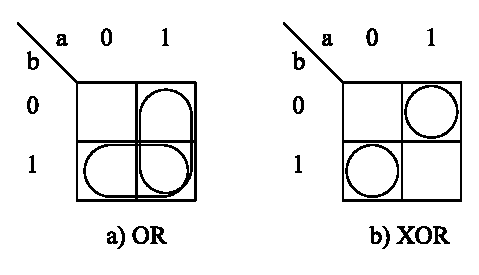
\epsfig{file=minterm.eps}
%\caption{Satisfying assignments for simple gates}
%  \label{ORXOR}
%\end{figure}
\newdef{definition11}{Definition}


%\subsection{Bounded Model Checking}

%Description of our algorithm will largely follow that of \textbf{bounded model checking (BMC)} \cite{SMCSAT},
%so we present here briefly how to check reachability in BMC.

%\newdef{definition11}{Definition}\label{KripkeStructure}
%\begin{definition11}
%\textbf{Kripke structure} is a 5-tuple $M=(S,I,T,A,L)$, with a finite set of states $S$,
%the set of initial states $I\subseteq S$,
%transition relation between states $T_{��}\subseteq S\times S$,
%and the labeling of the states $L:S\rightarrow 2^{A}$ with atomic propositions set $A$.
%\end{definition11}

%BMC is a model checking technology that consider only limited length path.
%We call this length as the bound of path.
%We denote the $i$-th and $i+1$-th state as $s_i$ and $s_{i+1}$,
%and transition relation between them as $T(s_i,s_{i+1})$.

%Let the safety property under verification be $ASSERT$,
%the goal of BMC is to find a state that violates $ASSERT$.
%Then BMC problem with bound $b$ can be expressed as:

%\begin{equation}\label{bmc}
%I(s_0)\wedge \bigwedge_{i=1}^{b-1} T(s_i,s_{i+1})\wedge \bigvee_{i=1}^{b}\neg ASSERT(s_i)
%\end{equation}

%Reduce formula (\ref{bmc}) into CNF format,
%and solve it with SAT solver,
%then a counterexample of length $b$ can be found if it exist.

\section{Checking Parameterized Complementary Assumption}\label{sec_checkUA}

In this section,
we will introduce how to check whether input sequence of circuit $E$ can be recovered from its output sequence.

\subsection{Parameterized Complementary Assumption}
\begin{figure*}[tb]
  \centering
  \leavevmode
  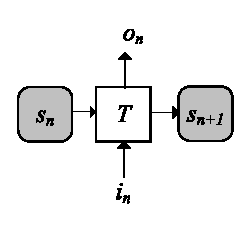
\epsfig{file=mealy.eps}
\caption{Unfolding Transition Function of Mealy Finite State Machine}
  \label{mealyfsm_unfolding}
\end{figure*}

Our algorithm cares about the input and output sequence of circuit $E$,
%so modeling such circuits with Kripke structure in definition \ref{KripkeStructure} isn't appropriate.
%On the other hand,
so \textbf{Mealy finite state machine}\cite{MEALY} is a suitable model for us.


\begin{definition11}\label{MealyFSM}\addtolength{\itemsep}{-0.5\baselineskip}
{\setlength{\baselineskip}{0.5\baselineskip}
\textbf{Mealy finite state machine} is a 6-tuple $M=(S,s_0,I,O,T,G)$,consisting of the following
\begin{enumerate}
\item A finite set of state $S$
\item An initial state $s_0\in S$
\item A finite set of input alphabets $I$
\item A finite set of output alphabets $O$
\item A state transition function $T: S\times I\to S$
\item An output function $G:S\times I\to O$
\end{enumerate}
}
\end{definition11}


The circuit $E$ can be modeled by such a Mealy finite state machine.
%as shown in figure \ref{mealyfsm_unfolding}a).
The relationship between its output sequence $o\in O^{\omega}$ and input sequence $i\in I^{\omega}$ is shown in figure \ref{mealyfsm_unfolding}.
This relationship is built by unfolding the transition function $T$ and output function $G$ $d$ times,
as shown in formula (\ref{unfolding}).

\begin{equation}\label{unfolding}
\bigwedge_{m=n}^{n+d-1} \Big\{ s_{m+1}\equiv T(s_m,i_m) \wedge  o_m\equiv G(s_m,i_m) \Big\}
\end{equation}

In order to recover $i\in I^{\omega}$ from $o\in O^{\omega}$,
we must know how to compute $i_n$ for every $n$,
that is, to find a function $f^{-1}$ that can compute $i_n$ from $o\in O^{\omega}$.

But due to the limited memory of realistic computers,
we can't take the infinite length sequence $o\in O^{\omega}$ as input to $f^{-1}$,
we can only use a finite length sub-sequence of $o$.
This sub-sequence has two parameters,
its length $l$ and its delay $d$ compared to $i_n$, as shown in following figure \ref{dl}.

Thus,
$f^{-1}:O^l\to I$ is now a boolean function that takes the finite length sequence $<o_{n+d-l},\dots , o_{n+d-1} >$ as input,
and computes $i_n$.

For a particular pair of $d$ and $l$,
$f^{-1}$ exists if the the following assumption holds:

\begin{definition11}\label{UniquenessAssumption}
\textbf{Parameterized Complementary Assumption}:For any valuation of sequence $<o_{n+d-l},\dots , o_{n+d-1} >$,
assume there exists no more than one valuation of $i_n$,
that can make formula (\ref{unfolding}) satisfiable.
\end{definition11}

This assumption holds if and only if the following formula (\ref{checkUA}) is unsatisfiable.

\begin{figure}[htbp]
  \centering
  \leavevmode
  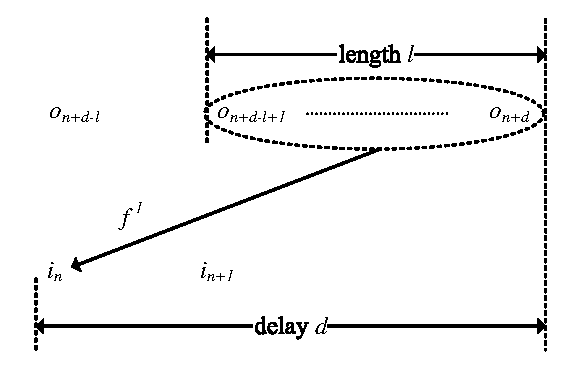
\epsfig{file=dl.eps}
\caption{$f^{-1}$ and its Parameters}
  \label{dl}
\end{figure}


\begin{equation}\label{checkUA}
\begin{array}{c}
\bigwedge_{m=n}^{n+d-1} \Big\{ s_{m+1}\equiv T(s_m,i_m)\wedge o_m\equiv G(s_m,i_m) \Big\} \wedge \\
\bigwedge_{m=n}^{n+d-1} \Big\{ s'_{m+1}\equiv T(s'_m,i'_m)\wedge o'_m\equiv G(s'_m,i'_m) \Big\} \wedge \\
\bigwedge_{m=n+d-l}^{n+d-1} o_m\equiv o'_m\wedge \\
i_n\ne i'_n
\end{array}
\end{equation}

In formula (\ref{checkUA}),
the first line is the same as formula (\ref{unfolding}),
the second line is a copy of formula (\ref{unfolding}),
except that its variables are all renamed by appending a prime.
These two lines mean two individual unfolding of circuit $E$.
The third line constrains their output sequences $<o_{n+d-l},\dots , o_{n+d-1} >$ and $<o'_{n+d-l},\dots , o'_{n+d-1} >$ to be the same,
and the fourth line constrains that their input alphabet $i_n$ and $i'_n$ are different.

For a particular pair of $d$ and $l$ , checking formula (\ref{checkUA}) may return two results:
\begin{enumerate}
\item \textbf{Satisfiable}. In this situation,
      for a $<o_{n+d-l},\dots , o_{n+d-1} >$,
      there exist two different $i_n$ and $i'_n$ that can both make formula (\ref{unfolding}) satisfiable.
      This violates definition \ref{UniquenessAssumption},
      so no $f^{-1}$ exists for this pair of $d$ and $l$.
      We should continue searching for larger $d$ and $l$.
\item \textbf{Unsatisfiable}.In this situation,
      the parameterized complementary assumption is satisfied,
      so a $f^{-1}:O^l\to I$ exists for this pair of $d$ and $l$.
      We will build $f^{-1}$ with formula (\ref{unfolding}) in section \ref{sec_buildF}.
\end{enumerate}


\subsection{Ruling out Invalid Input Alphabets with Assertion}\label{subsec_AST}

Most communication protocols and systems have some restrictions on valid pattern of input alphabet.
Assume that this restriction is expressed as an assertion predicate $R: I\to \{0,1\}$,
in which $R(i_{n})\equiv 0$ means that $i_n$ is an invalid input alphabet.
%More formally, assume the set of input boolean variables is $I_{var}$,
%then $I\subset 2^{I_{var}}$.
Invalid input alphabets will be mapped to some predefined error output alphabet,
that is,
for $i_n$,$i'_n\in \{i_m|R(i_m)\equiv 0\}$,
they will both be mapped to the same error output alphabet $e\in O$.
Hence, this will prevent our approach from distinguishing $i_n$ from $i'_n$.

Such restrictions are often documented clearly in specification of communication protocols,
%and can be found out easily.
so we chose to employ an assertion based mechanism,
such that the user can code these restrictions $R$ into their script or source code.

Thus, formula (\ref{unfolding}) and (\ref{checkUA}) should be rewritten as following formula (\ref{unfolding_ast}) and (\ref{checkUA_ast}),
in which bold formulas are used to account for predicate $R$.


\begin{equation}\label{unfolding_ast}
\bigwedge_{m=n}^{n+d-1}
\Big\{
s_{m+1}\equiv T(s_m,i_m) \wedge
o_m\equiv G(s_m,i_m) \wedge
\boldsymbol{R (i_m)}
\Big\}
\end{equation}

\begin{equation}\label{checkUA_ast}
\begin{array}{c}
\bigwedge_{m=n}^{n+d-1}
\Big\{ s_{m+1}\equiv T(s_m,i_m) \wedge o_m\equiv G(s_m,i_m) \wedge \boldsymbol{R (i_m)} \Big\} \wedge \\
\bigwedge_{m=n}^{n+d-1}
\Big\{ s'_{m+1}\equiv T(s'_m,i'_m) \wedge o'_m\equiv G(s'_m,i'_m) \wedge \boldsymbol{R (i'_m)} \Big\} \wedge \\
\bigwedge_{m=n+d-l}^{n+d-1} o_m\equiv o'_m \wedge \\
i_n\ne i'_n
\end{array}
\end{equation}

\subsection{Approximating Reachable State Set with Prefix Sequence}\label{subsec_Prfx}
In last subsection, we have constrained the valid pattern of $i_m$.
But $s_n$ in figure \ref{mealyfsm_unfolding} still hasn't been constrained yet.
This $s_n$ may be outside of reachable state set of circuit $E$,
which may make checking parameterized complementary assumption fail unnecessary.

Assume that circuit $E$ can be modeled by Mealy state machine $M_E=(S,s_0,I,O,T,G)$.
Its reachable state set with assertion predicate $R$ is:

\begin{equation}\label{rse}
\begin{split}
RS_E & \gets  \Big\{s|\exists q\textrm{ such that } \\
& s\equiv s_q\wedge \bigwedge_{m=0}^{q-1}\big\{
s_{m+1}\equiv T(s_m,i_m)\wedge R(i_m)
\big\}\Big\}
\end{split}
\end{equation}

Thus, to rule out unreachable $s_n$,
we need to rewrite formula (\ref{unfolding_ast}) and (\ref{checkUA_ast})
as formula (\ref{unfolding_ast_rs}) and (\ref{checkUA_ast_rs}) :


\begin{equation}\label{unfolding_ast_rs}
\begin{array}{c}
s_n\in RS_E \wedge \\
\bigwedge_{\boldsymbol{m=n}}^{n+d-1}
\Big\{
s_{m+1}\equiv T(s_m,i_m) \wedge
o_m\equiv G(s_m,i_m) \wedge
R (i_m)
\Big\}
\end{array}
\end{equation}

\begin{equation}\label{checkUA_ast_rs}
\begin{array}{c}
s_n\in RS_E \wedge s'_n\in RS_E \wedge \\
\bigwedge_{\boldsymbol{m=n}}^{n+d-1} \Big\{ s_{m+1}\equiv T(s_m,i_m) \wedge o_m\equiv G(s_m,i_m) \wedge R (i_m) \Big\} \wedge \\
\bigwedge_{\boldsymbol{m=n}}^{n+d-1} \Big\{ s'_{m+1}\equiv T(s'_m,i'_m) \wedge o'_m\equiv G(s'_m,i'_m) \wedge R (i'_m) \Big\} \wedge \\
\bigwedge_{m=n+d-l}^{n+d-1} o_m\equiv o'_m \wedge \\
i_n\ne i'_n
\end{array}
\end{equation}

%But computing reachable state set $RS_E$ for large scale circuit $E$ is a very expensive operation that we can't afford.

Now we have two extreme cases:
\begin{enumerate}
\item One extreme case is formula (\ref{unfolding_ast}) and (\ref{checkUA_ast}) with low computation complexity,
      but high risk of unnecessary fail in checking parameterized complementary assumption.
\item The other extreme case is formula (\ref{unfolding_ast_rs}) and (\ref{checkUA_ast_rs}),
      which are not affected by unreachable state set,
      but with very high computation complexity in computing reachable state set $RS_E$.
\end{enumerate}

Obviously, on the balance of these two extremes ,
we want a method with both acceptable computation complexity and
low risk of unnecessary fail in checking parameterized complementary assumption.

To achieve this,
we approximate $RS_E$ with a prefix state transition sequence of length $p$:

\begin{equation}\label{apprse}
\begin{split}
RS_E^p & \gets  \Big\{s| \\
& s\equiv s_n\wedge \bigwedge_{m=n-p}^{n-1}\big\{
s_{m+1}\equiv T(s_m,i_m)\wedge R(i_m)
\big\}\Big\}
\end{split}
\end{equation}

Obviously, formula (\ref{apprse}) is very similar to (\ref{rse}),
except that (\ref{apprse}) doesn't consider initial state $s_0$.
So $RS_E$ and all $RS_E^p$ form a total order relation :

\begin{displaymath}
RS_E\subseteq\dots \subseteq RS_E^p\subseteq\dots \subseteq RS_E^q\subseteq\dots \textrm{  where } p>q
\end{displaymath}

So now, in addition to parameters $d$ and $l$,
we have the third parameter $p$ to be searched.
In order to account for $RS_E^p$,
we need to rewrite formula (\ref{unfolding_ast}) and (\ref{checkUA_ast}) as
following formula (\ref{unfolding_ast_p}) and (\ref{checkUA_ast_p}),
by changing starting index of $m$ from $n$ to $n-p$:

\begin{equation}\label{unfolding_ast_p}
\begin{split}
\boldsymbol{F_E} &\gets \\
&
\bigwedge_{\boldsymbol{m=n-p}}^{n+d-1}
\Big\{
s_{m+1}\equiv T(s_m,i_m) \wedge
o_m\equiv G(s_m,i_m) \wedge
R (i_m)
\Big\}
\end{split}
\end{equation}

\begin{equation}\label{checkUA_ast_p}
\begin{array}{c}
%s_n\in RS_E^p \wedge s'_n\in RS_E^p \wedge \\
\bigwedge_{\boldsymbol{m=n-p}}^{n+d-1} \Big\{ s_{m+1}\equiv T(s_m,i_m) \wedge o_m\equiv G(s_m,i_m) \wedge R (i_m) \Big\} \wedge \\
\bigwedge_{\boldsymbol{m=n-p}}^{n+d-1} \Big\{ s'_{m+1}\equiv T(s'_m,i'_m) \wedge o'_m\equiv G(s'_m,i'_m) \wedge R (i'_m) \Big\} \wedge \\
\bigwedge_{m=n+d-l}^{n+d-1} o_m\equiv o'_m \wedge \\
i_n\ne i'_n
\end{array}
\end{equation}


\textbf{Now put it altogether},
with formula (\ref{unfolding_ast_p}) and (\ref{checkUA_ast_p}),
we iterate through all valuations of $d$, $l$ and $p$,
from smaller one to larger one,
until we find one valuation of $d$,$l$ and $p$ that makes formula (\ref{checkUA_ast_p}) unsatisfiable,
then that valuation and $F_E$ in formula (\ref{unfolding_ast_p}) will be used in section \ref{sec_buildF} to build complementary circuit $E^{-1}$.



\section{Building Complementary Circuit with ALLSAT Algorithm Designed for XOR Intensive Circuits}\label{sec_buildF}

If we find a proper value for parameters $d$,$l$ and $p$ in section \ref{sec_checkUA},
we can now build the complementary circuit $E^{-1}$'s boolean function $f^{-1}:O^l\to I$ in this section.


\subsection{Algorithm Framework}

According to section \ref{subsec_Prfx},
$f^{-1}:O^l\to I$ can be built from formula (\ref{unfolding_ast_p})
by enumerating satisfying assignments of $<o_{n+d-l},\dots , o_{n+d-1} >$ and $i_n$.

Assume that the set of all total satisfying assignments of formula (\ref{unfolding_ast_p}) is $\{A_1,\dots ,A_t\}$,
then $f^{-1}$ can be defined as:

\begin{displaymath}
\begin{split}
f^{-1} & (<o_{n+d-l},\dots , o_{n+d-1} >) = \\
&
\left\{ \begin{array}{llll}
A_1(i_n) & & if & \bigwedge_{m=n+d-l}^{n+d-1}o_m\equiv A_1(o_m) \\
& \dots & & \\
A_t(i_n) & & if & \bigwedge_{m=n+d-l}^{n+d-1}o_m\equiv A_t(o_m)
\end{array}
\right.
\end{split}
\end{displaymath}


But this naive approach suffers from the state space explosion problem.
For $O^l$ that contains $m$ boolean variables,
there may be $2^m$ satisfying assignments,
which make it impossible to build $f^{-1}$ for large $m$.

There exists some much more efficient approaches
to enumerate satisfying assignments of SAT instance
\cite{PRIMECLAUSE,SATUNBMC,MINASS,EFFCON,MINCEX,MEMEFFALLSAT,REPARAM,EFFSATUSMCCO}.
%including one invented by us\cite{MINCEX}.
Their basic idea has been introduced in subsection \ref{subsec_ALLSAT}.

But these approaches are still not efficient enough for our application.
The essential reason that leads to this inefficiency
is the wide usage of XOR gates in communication and arithmetic circuits.
As explained in subsection \ref{subsec_ALLSAT},
satisfying assignments of XOR can't be minimized.

So we invent a novel approach that is specially designed for XOR intensive circuits,
as shown below:

\begin{algo}\label{buildfdec_frm}
\textbf{Synthesizing Complementary Circuit}
\begin{enumerate}\addtolength{\itemsep}{-0.5\baselineskip}
{\setlength{\baselineskip}{0.5\baselineskip}
\item assume that $\boldsymbol{I_{var}}$ and $\boldsymbol{O_{var}}$ are respectively boolean variable sets that represent $i_n$ and $<o_{n+d-l},\dots , o_{n+d-1} >$.
      and $\boldsymbol{F_E}$ is defined in  formula (\ref{unfolding_ast_p})
\item $G_{XOR}\gets \{\}$
\item foreach $v\in I_{var}$ \{
\item \hspace{0.3cm} $SA_v\gets \{\}$
\item \hspace{0.3cm} while ( $F_E\wedge v\equiv 1$ is satisfiable) \{
\item \hspace{0.6cm} Assume $A$ is a satisfying assignment
\item \hspace{0.6cm} $\boldsymbol{A_{BFL}\gets BFL(F_E,A,v)}$
\item \hspace{0.6cm} $\boldsymbol{\{A_{XOR},G\}\gets XORMIN(F_E, A_{BFL},v)}$
\item \hspace{0.6cm} $SA_v\gets SA_v \cup \{ A_{XOR} \}$
\item \hspace{0.6cm} $G_{XOR}\gets G_{XOR}\cup G$
\item \hspace{0.6cm} $F_E\gets F_E\wedge bcls_{A_{XOR}}$
\item \hspace{0.6cm} $F_E\gets F_E\wedge \bigwedge _{(x_1\gets v_1\oplus v_2)\in G}\{x_1\equiv v_1\oplus v_2\}$
\item \hspace{0.3cm} \}
\item \hspace{0.3cm} Building $f^{-1}_v:\{0,1\}^{O_{var}}\to \{0,1\}$ for $v\in I_{var}$
\item \}
\item Building $f^{-1}: \{0,1\}^{O_{var}}\to \{0,1\}^{I_{var}}$
}
\end{enumerate}
\end{algo}

In line 2, $G_{XOR}$ is a set of XOR gates discovered by XORMIN on line 8.
It will help to speedup the process of enumerating satisfying assignments of $F_E\wedge v\equiv 1$ on line 5.
More details will be given in subsection \ref{subsec_XOR}.

Line 3 will iterate through all input boolean variables $v\in I_{var}$,
and build a function $f^{-1}_v$ for it in \textbf{line 14},
$f^{-1}$ can be built from all such $f^{-1}_v$ in \textbf{line 16}.
The detail of building $f^{-1}_v$ and $f^{-1}$ will be given in subsection \ref{build_F}.

In line 4,
$SA_v$ is a set of satisfying assignments that can make $v\equiv 1$,
this set will be used in line 14 to build $f^{-1}_v$.

In line 5,
we will iterate through all satisfying assignments $A$ of $F_E\wedge v\equiv 1$,
and minimize them in two steps.
\begin{enumerate}
\item \textbf{BFL} in line 7
is a modified BFL\cite{MINASS} that will be described in subsection \ref{subsec_BFL}.
\item \textbf{XORMIN} in line 8 will further minimize the result of BFL by discovering hidden XOR gates,
and return the minimized assignment $A_{XOR}$ and discovered XOR gate set $G$.
This is one of our major contributions,
and will be described in subsection \ref{subsec_XOR}.
\end{enumerate}

In line 11,
we will rule out the enumerated satisfying assignment $A_{XOR}$ by adding its blocking clauses into $F_E$.

In line 12,
we will add clauses to $F_E$ for newly discovered XOR.

\subsection{Minimizing Satisfying Assignments with Modified BFL algorithm}\label{subsec_BFL}

The basic idea of BFL has been introduced in subsection \ref{subsec_ALLSAT},
so we present the modified BFL here directly.

\begin{algo}
\textbf{BFL($F_E$,$A$,$v$)}
\begin{enumerate}\addtolength{\itemsep}{-0.5\baselineskip}
{\setlength{\baselineskip}{0.5\baselineskip}
\item Assume $\boldsymbol{O_{var}}$ is boolean variable set that represents $<o_{n+d-l},\dots , o_{n+d-1} >$
\item foreach $u\in O_{var}$ \{
\item \hspace{0.5cm}  if($\boldsymbol{F_E\wedge \neg v\wedge A|_{O_{var} -\{u\}}}$ \textbf{is unsatisfiable})  \{
\item \hspace{1.0cm}     $A\gets A|_{O_{var} -\{u\}}$
\item \hspace{1.0cm}     $O_{var} \gets O_{var} -\{u\}$
\item \hspace{0.5cm} \}
\item \}
\item return $A$
}
\end{enumerate}
\end{algo}

In line 2,
we iterate through all output variable $u\in O_{var}$.

In line 3,
if that formula is unsatisfiable,
then $A|_{O_{var} -\{u\}}$ is sufficient to lead to $v\equiv 1$.
Thus, we can remove assignment of $u$ from $A$.

According to subsection \ref{subsec_ALLSAT},
for circuits with lots of XOR gates,
BFL can't minimize its satisfying assignments.
Thus, algorithm \ref{buildfdec_frm} can't terminate in reasonable time for large XOR intensive circuits.

\subsection{Minimizing Satisfying Assignments by Discovering XOR gates}\label{subsec_XOR}

%In order to overcome the problem of BFL,
%we need to discover XOR hidden in result of BFL.
%by checking \textbf{XOR pairing assumption} below.

%\begin{definition11}\label{XORpairingass}
%\textbf{XOR pairing assumption}:
%For a formula $F$ over boolean variable set $V$,
%a variable $v\in V$ that should always be 1,
%and one satisfying assignments $A_F$ of $F_E\wedge v$,
%assume there is another satisfying assignment $A'_F$,
%such that only two variables $v_1$ and $v_2$ have difference assignment in $A_F$ and $A'_F$ ,
%that is,
%$\{v_i|A_F(v_i)\ne A'_F(v_i)\}\equiv \{v_1,v_2\}$,
%\end{definition11}

Intuitively, assume that the circuit in figure \ref{rmxor}a) has an input variable set $V=\{v_1,v_2,v_3,\dots,v_n\}$,
and it \textbf{MAY} contain a XOR $v'\gets v_1\oplus v_2$.
We can avoid enumerating the assignments of $v_1$ and $v_2$ %by moving this XOR out of the circuit,
%and enumerate assignments of $V\cup\{x_1\}-\{v_1,v_2\}=\{\boldsymbol{x_1},v_3,...,v_n\}$.
by first checking the existence of this XOR,
and then,
as shown in figure \ref{rmxor}b),
if this XOR actual exists,
we add another XOR $x_1\gets v_1\oplus v_2$ into this circuit,
and enumerate assignments on $V\cup \{x_1\}-\{v_1,v_2\}$ instead of $V$.


\begin{figure}[htbp]
  \centering
  \leavevmode
  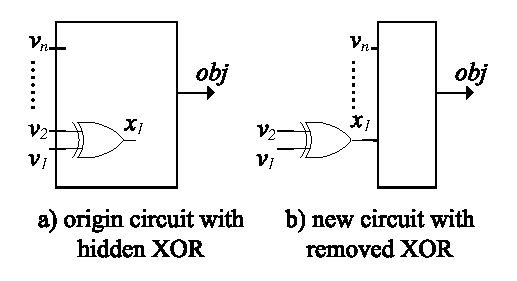
\epsfig{file=xor.eps}
\caption{Discovering Hidden XOR}
  \label{rmxor}
\end{figure}

%In order to remove this XOR,
%we must first make sure that there actually exists a XOR in this circuit.

Formally, to check existence of XOR $v'\gets v_1\oplus v_2$,
for a satisfying assignment $A_F$ of formula $F_E$,
we define a new assignment $A_{x_1}$ in formula (\ref{mergeA}),
by first removing assignments of $v_1$ and $v_2$ from $A_F$,
and then adding assignment of $x_1$ as result of XORing $v_1$ and $v_2$ into $A_F$.

\begin{equation}\label{mergeA}
A_{x_1}\gets A_F|_{O_{var}-\{v_1,v_2\}}|^{x_1\gets A_F(v_1)\oplus A_F(v_2)}
\end{equation}

With this $A_{x_1}$,
existence of $v'\gets v_1\oplus v_2$ can be decided by checking unsatisfiability of the following formula :

\begin{equation}\label{check_XPA}
F_E\wedge \neg v\wedge A_{x_1}\wedge \{x_1\equiv v_1\oplus v_2\}
\end{equation}

Unsatisfiable of formula (\ref{check_XPA}) means that $A_{x_1}$ can't make $v$ to be 0,
so $A_{x_1}$ must be a satisfying assignment of $F_E\wedge v\wedge \{x_1\equiv v_1\oplus v_2\}$.

Thus,
$A_F$ and $A_F|_{V-\{v_1,v_2\}}|^{v_1\gets \neg A_F(v_1)}|^{v_2\gets \neg A_F(v_2)}$,
that can't be merged by BFL,
have now been merged into $A_{x_1}$ with the help of a newly discovered XOR gate $x_1\gets v_1\oplus v_2$.
If we repeatedly merge assignments by checking unsatisfiability of formula (\ref{check_XPA}),
we can get a partial assignment of $F_E\wedge v\wedge \{x_1\equiv\dots\oplus\dots\}\dots\wedge \{x_n\equiv\dots\oplus\dots\}$ in formula (\ref{ax1xn}),
which contains $2^n$ total assignments,
that can't be merged by BFL.

\begin{equation}\label{ax1xn}
A_{x_1\dots x_n}\gets A_F|_{O_{var}-\{v_1,\dots\}}|^{x_1\gets \dots\oplus\dots}\dots|^{x_n\gets \dots\oplus\dots}
\end{equation}

With above discussion in mind, we describe \textbf{XORMIN} below:



\begin{algo}\label{buildfdec}
\textbf{ $\boldsymbol{XORMIN(F_E, A_F,v)}$}
\begin{enumerate}\addtolength{\itemsep}{-0.5\baselineskip}
{\setlength{\baselineskip}{0.5\baselineskip}
\item $G=\{\}$
\item do \{

\item \hspace{0.3cm} $G_{new}=\{\}$  // the set of newly discovered XOR
%\item \hspace{0.3cm} assume the set of variables in $A_F$ is $V$
\item \hspace{0.3cm} foreach $v_1,v_2\in O_{var}$ \{

\item \hspace{0.6cm}   if(\textbf{formula (\ref{check_XPA}) is unsatisfiable})\{

\item \hspace{0.9cm}     $G_{new}\gets G_{new}\cup \{ x_1\gets v_1\oplus v_2\}$
\item \hspace{0.9cm}     $A_F\gets A_F|_{O_{var}-\{v_1,v_2\}}|^{x_1\gets A_F(v_1)\oplus A_F(v_2)}$
\item \hspace{0.9cm}     $O_{var}\gets O_{var}\cup \{x_1\}-\{v_1,v_2\}$
\item \hspace{0.9cm}     $F_E\gets F_E\wedge bcls_{A_F}$
\item \hspace{0.9cm}     $F_E\gets F_E\wedge \bigwedge _{\{x_1\gets v_1\oplus v_2\}\in G_{new}}\big\{x_1\equiv v_1\oplus v_2\big\}$

\item \hspace{0.6cm}   \}
\item \hspace{0.3cm} \}
\item \hspace{0.3cm} $G=G\cup G_{new}$
\item \} while($G_{new}\ne \{\}$)
\item return $\{A_F,G\}$
}
\end{enumerate}
\end{algo}

In line 1,
$G$ is an empty set that will be used to hold all XOR gates discovered by this algorithm.

In line 2, the do-while statement will repeatedly discover new XOR gates,
until no more XOR gates can be discovered.

In line 4,
foreach statement will enumerate each pair of $v_1,v_2\in V$,
and line 5 will test if there is a XOR gate between $v_1$ and $v_2$.



\subsection{Building $f^{-1}_v$ and $f^{-1}$}\label{build_F}

The complementary function $f^{-1}:O^l\to I$ is the function that takes $<o_{n+d-l},\dots , o_{n+d-1} >$
, and computes $i_n$ .
Assume that $i_n$ is represented by boolean variable set $I_{var}$,
and $<o_{n+d-l},\dots , o_{n+d-1} >$ is represented by boolean variable set $O_{var}$.

Thus, $f^{-1}$ in boolean domain is $f^{-1}:\{0,1\}^{O_{var}}\to \{0,1\}^{I_{var}}$.
Then building $f^{-1}$ can be partitioned into multiple tasks,
each task builds a boolean function $f^{-1}_v: \{0,1\}^{O_{var}}\to \{0,1\}$ for a $v\in I_{var}$.

To build $f^{-1}_v$,
let's assume that $SA_v$ is the set of satisfying assignments that makes $v$ to take on 1.
Then $f^{-1}_v$ can be defined as :

\begin{displaymath}
f^{-1}_v(x) = \left\{ \begin{array}{lll}
1 & & \exists A\in SA_v.st. x\equiv A(x) \\
0 & & else
\end{array}
\right.
\end{displaymath}

\section{Experimental Results}
\subsection{Benchmarks}
\begin{table}[tb]
\centering
\caption{Information of Benchmarks}
\begin{tabular}{|c|c|c|c|c|c|}
\hline
&XGXS&XFI&66 bits&PCIE&T2 et-\\
&&&scrambler&&hernet\\\hline
Line number&&&&&\\
of verilog&214&466&24&1139&1073\\
source code&&&&&\\\hline
Number of&15&135&58&22&48\\
registers&&&&&\\ \hline
Data path&8&64&66&10&10\\
width&&&&&\\ \hline
\end{tabular}
\end{table}

\begin{table}[tb]
\centering
\caption{Results of Checking Parameterized Complementary Assumption}
\begin{tabular}{|c|c|c|c|c|c|}
\hline
&XGXS&XFI&66 bit&PCIE&T2 et-\\
&&&scrambler&&hernet\\ \hline
run time&0.51&71.60&2.51&32.74&44.48\\
(seconds)&&&&&\\\hline
$d$      &1       &0     &0         &2   &4          \\ \hline
$p$      &0       &3     &1         &1   &0          \\ \hline
$l$      &1       &2     &2         &1   &1          \\ \hline
\end{tabular}
\end{table}

Our approach is the first one that can synthesize complementary circuits automatically,
so we can't compare it with other research results.

Temporal logic synthesis is a research topic that is somewhat close to us,
but it can't be scaled to large circuits,
and no commercial available IP cores are written in temporal logic.
Thus, it's impossible to compare our results with temporal logic synthesis.

\begin{table*}[tb]
\centering
\caption{Results of Building Complementary Circuits}
\begin{tabular}{|c|c|c|c|c|c|c|}
\hline
       &                 &XGXS&XFI& 66 bit   &PCIE&T2 ethernet	  \\
       &                 &       &      & scrambler&    &        	  \\ \hline
BFL    &run time(seconds)&32.67  &$>10,000$&8.56   &$>10,000$&$>10,000$	 	     \\ \cline{2-7}
only   &line number of   &2927   &N/A   &11882     &N/A &N/A 		     \\
       &generated verilog&       &      &          &    &        	  \\ \hline
BFL+   &run time         &1.52   &2939.47&11.97     &47.55&36.64        	  \\ \cline{2-7}
XORMIN &line number of   &1525   &48829 &4723      &11254& 16616       	  \\
       &generated verilog&       &      &          &    &        	  \\ \hline
\end{tabular}
\end{table*}

Table 1 shows some information of following benchmarks.
\begin{enumerate}
  \item The first benchmark is a XGXS encoder that is compliant to clause 48 of IEEE-802.3ae 2002 standard \cite{IEEE80232002}.
  \item The second benchmark is a XFI encoder that is compliant to clause 49 of the same IEEE standard.
  \item The third benchmark is a 66 bit scrambler that is used to make a data sequence to have enough transitions between 0 and 1,
        such that it can run through high speed noisy serial transmission channel.
  \item The fourth benchmark is a PCIE physical coding module.
  \item The fifth benchmark is Ethernet module of Sun's OpenSparc T2 processor.
\end{enumerate}


\subsection{Experimental Results}

Table 2 shows the run time of checking parameterized complementary assumption on these circuits,
and the discovered proper values of parameters.

Table 3 shows the results of generated verilog description of complementary circuits.
With \textbf{BFL only}, complementary circuits of the three most complex circuits:
XFI, PCIE and T2 ethernet,
can't be built within 10,000 seconds.
While with \textbf{BFL and XORMIN}, we can finally build all complementary circuits successfully within 3000 seconds.

These generated complementary circuits are all been verified by dynamic simulations.


\section{Related Works}
\subsection{Temporal Logic Synthesis}
Automatically synthesis of program from logic specification is first identified as Church's problem in 1962\cite{LOGARTHAUTO}.
Some early researches \cite{SLVSQFSS,AUTOINF} solve this problem by reducing it to checking emptiness of tree automata.

With the invention of temporal logic in the early 1980s,
this problem was considered again \cite{DSGSYNTMPLG,SYNTMPLGSPC}.
But in 1989, A. Pnueli and R. Rosner\cite{SYNRCTVMD} pointed out that the complexity of LTL synthesis was double exponent in the size of the formula.

This high complexity drives researchers turning their focus on finding smaller but still useful subset of temporal logic,
such that synthesis problem can be solved with lower complexity.

One line of research \cite{CNTLSYNTMDAUTO,DTMGENGMELTL,SYNRCTVDES} focused on the so-called generalized reactive formulas of the form:
$(\square \lozenge p_1 \wedge \cdots \square \lozenge p_m) \to (\square \lozenge q_1 \wedge \cdots \square \lozenge q_n)$.
Complexity of solving synthesis problem for such formula is $O(N^3)$.

The other line of research focused on finding efficient symbolic algorithm \cite{SYNCNTLBNDRPN}
for expensive safra determination algorithm \cite{CMPLXAUTO} on a useful formula subset,
or just avoiding it\cite{NEWALGSTRGSYN}.

\subsection{Satisfying Assignments Enumeration}

%There are two research directions for satisfying assignments enumeration.
%One is bottom up,
%which removes irrelevant variables from total assignments.
%The other is top down,
%which adds relevant variable's assignments into an empty set,
%to form a smaller and smaller assignment set.

ALLSAT algorithms all try to enlarge total satisfying assignment by removing irrelevant variables from total satisfying assignment,
such that a large cube that contains more total satisfying assignment can be obtained.

The first such approach is proposed by K. L. McMillan \cite{SATUNBMC}.
He constructs an alternative implication graph in SAT solver,
which records the reasoning relation that leads to the assignment of a particular object variable $obj$.
All variables outside this graph can be ruled out from the total assignment.
Kavita Ravi et al.\cite{MINASS} and P. P. Chauhan et al.\cite{REPARAM} remove those variables that can make $obj\equiv 0$ satisfiable one by one.
Shen et al.\cite{MINCEX} and HoonSang Jin et al.\cite{PRIMECLAUSE,EFFCON} use a conflict analysis based approach,
to remove multiple irrelevant variables in one SAT run.
Orna Grumberg et al.\cite{MEMEFFALLSAT} separates the variable set into important subset and non-important subset.
Variables in important subset have higher decision priority than non-important ones.
Thus,
the important subset form a search tree,
each leaf is another search tree for non-important set.
%Tobias Nopper et al.\cite{CMPMINCEX} propose an counterexample minimization algorithm for incomplete designs that contain black box.
Cofactoring \cite{EFFSATUSMCCO} qualifies out non-important variables by setting them to constant value returned by SAT solver.

\subsection{AND-XOR Logic Synthesis}

Classical logic synthesis works on AND-OR network.
Its kernel is two-level logic minimization,
which tries to find a small sum-of-products expression for boolean function $f$.
It is obvious that such two-level logic minimization algorithms are very similar to satisfying assignments enumeration described in previous subsection,
except that they don't work on SAT solvers.

Three most well known two-level logic minimization algorithms are Quine-McCluskey\cite{McCluskey},
Scherzo\cite{Scherzo},
and Espresso-II\cite{Espresso}.

Just like state-of-the-art ALLSAT that can't deal with XOR-intensive circuits efficiently,
classical logic synthesis also has the same problem.
So many researchers propose synthesis algorithms that target XOR-intensive circuits.

One research direction focuses on extending classical two-level AND-OR minimization to two-level AND-XOR network \cite{Mod2sum,ANDEXOR}.
These works normally describe circuits with most general ESOP (exclusive sum of product) expressions.
But very high computation complexity of these approaches prevents them from handling large circuits.

Another line of research relies on Reed-Muller expansion\cite{Reed},
one of its most used variant is Fixed Polarity Reed-Muller Form (FPRM) given by Davio and Deschamps\cite{FPRM},
in which a variable can have either positive or negative polarity.
Some related works that rely on FPRM are  \cite{fastexactFPRM,fastOFDD,lowpowerXOR}.

\section{Conclusions and Future Works}

In this paper,
we propose the first fully automatic approach that synthesizes complementary circuits for communication applications.
According to experimental results,
our approach can synthesize correct complementary circuits for many very complex circuits, including but not limited to PCIE and Ethernet.

One possible future work is to automatically generate assertions that rule out invalid input data patterns,
such that the users can be free from the burden of inspecting documentation and writing assertions.

Another possible future work is to deal with circuits with memory array and multiple clocks,
such that more complex communication mechanism,
such as data link layer and transaction layer,
can be dealt with by our approach.
%\end{document}  % This is where a 'short' article might terminate

%ACKNOWLEDGMENTS are optional
\section{Acknowledgments}
This project 60603088 is supported by National Natural Science Foundation of China ,
and Supported by the Program for Changjiang Scholars and Innovative Research Team in University No IRT0614.
Thanks to anonymous reviewers for their effort in reviewing this paper.

%This section is optional; it is a location for you
%to acknowledge grants, funding, editing assistance and
%what have you.  In the present case, for example, the
%authors would like to thank Gerald Murray of ACM for
%his help in codifying this \textit{Author's Guide}
%and the \textbf{.cls} and \textbf{.tex} files that it describes.

%
% The following two commands are all you need in the
% initial runs of your .tex file to
% produce the bibliography for the citations in your paper.
\bibliographystyle{abbrv}
%\bibliography{sigproc}  % sigproc.bib is the name of the Bibliography in this case
% You must have a proper ".bib" file
%  and remember to run:
% latex bibtex latex latex
% to resolve all references
%
% ACM needs 'a single self-contained file'!
%


\begin{thebibliography}{1}


\bibitem{IEEE80211N}
Chris Kozup.
Is 802.11n Right for You?
Mobility blog.
%Retrieved April 27, 2009, from http://blogs.cisco.com/wireless/comments/is\_80211n\_right\_for\_you/,
2008.

\bibitem{BRHDVD}
Stephen J. Dubner.
What Are the Lessons of the Blu-Ray/HD-DVD Battle? A Freakonomics Quorum.
The New York Times.
%Retrieved April 27, 2009, from  %http://freakonomics.blogs.nytimes.com/2008/03/04/what-are-the-lessons-of-the-blu-rayhd-dvd-battle-a-freakonomics-quorum/,
2008.

\bibitem{CHAFF}
M. Moskewicz, C. F. Madigan, Y. Zhao, L. Zhang, and S. Malik.
Chaff: Engineering an efficient SAT solver.
In DAC'01,
pp 530-535,
2001.

%\bibitem{BERKMIN}
%Evgueni Goldberg, Yakov Novikov.
%BerkMin: a fast and robust sat-solver.
%in DATE'02,
%pp 142-149,
%2002.

%\bibitem{EXTSAT}
%Niklas E�n, Niklas S�rensson.
%An Extensible SAT-solver.
%in SAT'03
%pp 502-518,
%2003.

%\bibitem{VERPROOF}
%Evguenii I. Goldberg, Yakov Novikov.
%Verification of Proofs of Unsatisfiability for CNF Formulas.
%in proceeding of DATE 2003, 10886-10891.

%\bibitem{VALIDSAT}
%Lintao Zhang, Sharad Malik.
%Validating SAT Solvers Using an Independent Resolution-Based Checker: Practical Implementations and Other Applications.
%in proceeding of DATE 2003, 10880-10885.

%\bibitem{SATLOGICMIN}
%Samir Sapra, Michael Theobald, Edmund M. Clarke.
%SAT-Based Algorithms for Logic Minimization.
%in ICCD'03,
%pp 510-519,
%2003.

\bibitem{PRIMECLAUSE}
HoonSang Jin , Fabio Somenzi.
Prime clauses for fast enumeration of satisfying assignments to boolean circuits.
In DAC'05,
pp 750-753,
2005.

%\bibitem{CMPMINCEX}
%Tobias Nopper, Christoph Scholl, Bernd Becker.
%Computation of minimal counterexamples by using black box techniques and symbolic methods.
%In ICCAD'07,
%pp 273-280,
%2007.

\bibitem{SATUNBMC}
K. L. McMillan.
Applying SAT methods in unbounded symbolic model checking.
In CAV'02,
pp 250-264,
2002.

\bibitem{MINASS}
Kavita Ravi, Fabio Somenzi.
Minimal Assignments for Bounded Model Checking.
In TACAS'04,
pp 31-45,
2004.

\bibitem{EFFCON}
H. Jin, H. Han, and F. Somenzi.
Efficient conflict analysis for finding all satisfying assignments of a Boolean circuit.
In TACAS'05,
pp 287-300,
2005.

\bibitem{MINCEX}
ShengYu Shen, Ying Qin, Sikun Li.
Minimizing Counterexample with Unit Core Extraction and Incremental SAT.
In VMCAI'05,
pp 298-312,
2005.

\bibitem{MEMEFFALLSAT}
Orna Grumberg, Assaf Schuster, Avi Yadgar.
Memory Efficient All-Solutions SAT Solver and Its Application for Reachability Analysis.
In FMCAD'04,
pp 275-289,
2004.

\bibitem{REPARAM}
P. P. Chauhan, E. M. Clarke, and D. Kroening.
A SAT-based algorithm for reparameterization in symbolic simulation.
In DAC'04,
pp 524-529,
2004.

%\bibitem{SMCSAT}
%A. Biere, A. Cimatti, E.M. Clarke, M. Fujita, Y. Zhu .
%Symbolic Model Checking using SAT procedures instead of BDDs.
%In DAC'99),
%pp 317-320,
%1999.

\bibitem{IEEE80232002}
IEEE Std. 802.3ae-2002. Amendment to IEEE Std 802.3-2002

\bibitem{LOGARTHAUTO}
Alonzo Church.
Logic,Arithmetic and Automata.
International Congress of Mathematicians,
pp 23-35,
1962

\bibitem{SLVSQFSS}
J.R. Buchi and L.H. Landweber.
Solving sequential conditions by finite-state strategies.
Transaction American Mathematic Society, Vol 138:295-311,
1969.

\bibitem{AUTOINF}
M.O. Rabin.
Automata on Infinite Objects and Church's Problem,
volume 13 of Regional Conference Series in Mathematics.
American Mathematic Society, 1972.

\bibitem{DSGSYNTMPLG}
E.M. Clarke and E.A. Emerson.
Design and synthesis of synchronization skeletons using branching time temporal logic.
In IBM Workshop on Logics of Programs,LNCS 131,
pp 52-71,
1981.
%\balancecolumns
\bibitem{SYNTMPLGSPC}
Z. Manna and P. Wolper.
Synthesis of communicating processes from temporal logic specifications.
ACM Trans. Prog. Lang. Sys., 6:68-93, 1984.

\bibitem{SYNRCTVMD}
A. Pnueli and R. Rosner.
On the synthesis of a reactive module.
In Proc. 16th ACM Symp. Princ. of Prog. Lang.,pages 179-190, 1989.

\bibitem{CNTLSYNTMDAUTO}
E. Asarin, O. Maler, A. Pnueli, and J. Sifakis.
Controller synthesis for timed automata.
In IFAC Symposium on System Structure and Control, pages 469-474. Elsevier, 1998.

\bibitem{DTMGENGMELTL}
R. Alur and S. La Torre.
Deterministic generators and games for LTL fragments.
ACM Trans. Comput. Log., 5(1):1-25,2004.


\bibitem{SYNRCTVDES}
N. Piterman, A. Pnueli and Y. Saar,
Synthesis of Reactive(1) Designs,
in VMCAI'06,
pp 364-380,
2006.

\bibitem{CMPLXAUTO}
S. Safra.
Complexity of Automata on Infinite Objects.
PhD thesis, The Weizmann Institute of Science, Rehovot, Israel, March 1989.

\bibitem{NEWALGSTRGSYN}
Aidan Harding, Mark Ryan, and Pierre-Yves Schobbens.
A New Algorithm for Strategy Synthesis in LTL Games.
in TACAS'05,
pp 477-492,
2005.

\bibitem{SYNCNTLBNDRPN}
Oded Maler, Dejan Nickovic and Amir Pnueli.
On Synthesizing Controllers from Bounded-Response Properties.
In CAV'07,
pp 95-107,
2007.

%\bibitem{ANZU}
%Barbara Jobstmann, Stefan Galler, Martin Weiglhofer, Roderick Paul Bloem.
%Anzu: A Tool for Property Synthesis.
%in CAV'07,
%pp 258-262,
%2007.

%\bibitem{OPTLTLSYN}
%Barbara Jobstmann, Roderick Bloem.
%Optimizations for LTL Synthesis.
%in FMCAD'06,
%pp 117-124,
%2006.

\bibitem{EFFSATUSMCCO}
M. K. Ganai, A. Gupta, and P. Ashar.
Efficient SAT-based unbounded symbolic model checking using circuit cofactoring.
In ICCAD'04,
pp 510-517,
2004.

\bibitem{MEALY}
Mealy, George H.
A Method for Synthesizing Sequential Circuits.
Bell Systems Technical Journal v 34, pp1045-1079, 1955.

\bibitem{McCluskey}
E.J. McCluskey.
Logic Design Principles.
Prentice-Hall,
1986.

\bibitem{Scherzo}
O. Coudert.
On solving covering problems.
In DAC'96,
1996.

\bibitem{Espresso}
R. Rudell and A. Sangiovanni Vincentelli.
Multiple valued minimization for PLA optimization.
IEEE Transactions on CAD,6(5),
pp 727-750,
1987.

\bibitem{Mod2sum}
P.W. Besslich and M. Riege.
An efficient program for logic synthesis of Mod-2 Sum Expressions.
In Euro ASIC'91,
pp 136-141,
1991.

\bibitem{ANDEXOR}
T. Sasao.
AND-EXOR expressions and their optimization.
Kluwer Academic Publishers,
Editor,
Logic Synthesis and Optimization,
Boston,
1993.

\bibitem{Reed}
I. Reed.
A class of multiple-error-correcting codes and their decoding scheme.
IRETrans. on Inf. Theory, PGIT-4:48-49,
1954.

\bibitem{FPRM}
M. Davio, Y. Deschamps, and A. Thayse.
Discrete and switching Functions.
George and McGraw-Hill, NY,
1978.

\bibitem{fastexactFPRM}
A. Sarabi and M. Perkowski.
Fast exact and quasi-minimal minimization of highly testable Fixed-Polarity AND/XOR canonical networks.
In DAC'92,
pp 30-35,
1992.

\bibitem{fastOFDD}
Rolf Drechsler, Bernd Becker, Michael Theobald.
Fast OFDD based minimization of fixed polarity Reed-Muller expressions.
in EURO-DAC,
1994.

\bibitem{lowpowerXOR}
Unni Narayanan and C. L. Liu.
Low power logic synthesis for XOR based circuits.
in ICCAD'97,
pp 570-574,
1997.

\end{thebibliography}

%APPENDICES are optional
%\balancecolumns
% That's all folks!
\end{document}
